\section*{Semantyczne reprezentacje wektorów cech modeli ASR}
\FloatBarrier
\subsection*{Analiza enkodowania znaczenia semantycznego mowy}

\begin{figure}[!htbp]
    \centering
    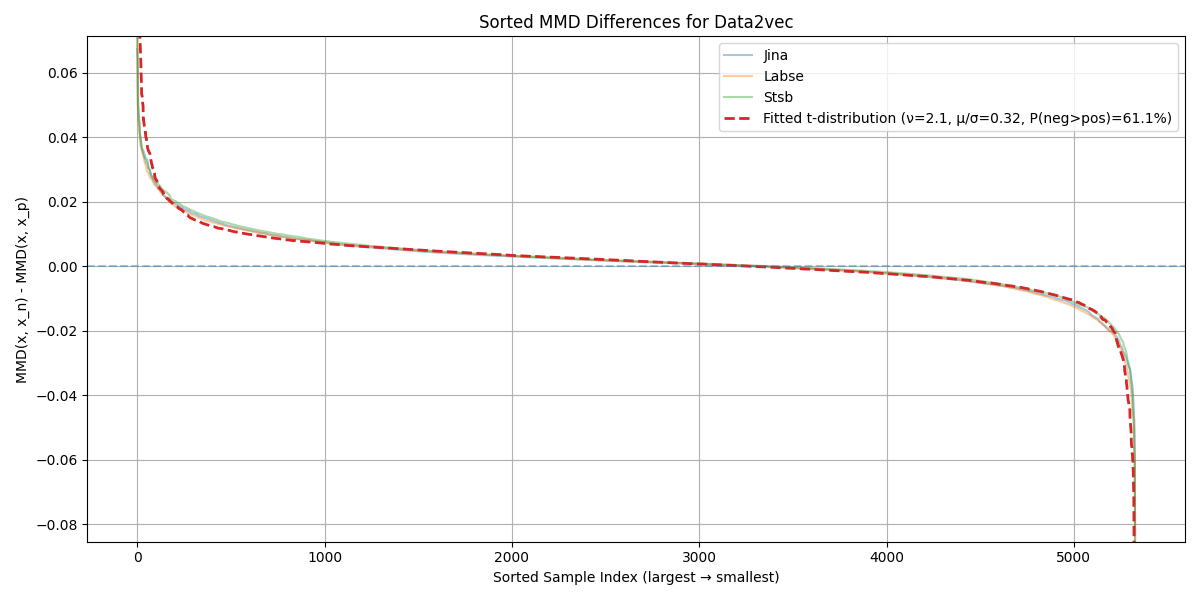
\includegraphics[width=0.8\linewidth]{figures/semantics/data2vec.png}
    \caption{Rozkład wartości różnicy podobieństw dla Data2Vec w ramach zbioru \textit{Medical Speech, Transcription, and Intent}}
    \label{fig:latent:medicalData2Vec}
\end{figure}

\begin{figure}[!htbp]
    \centering
    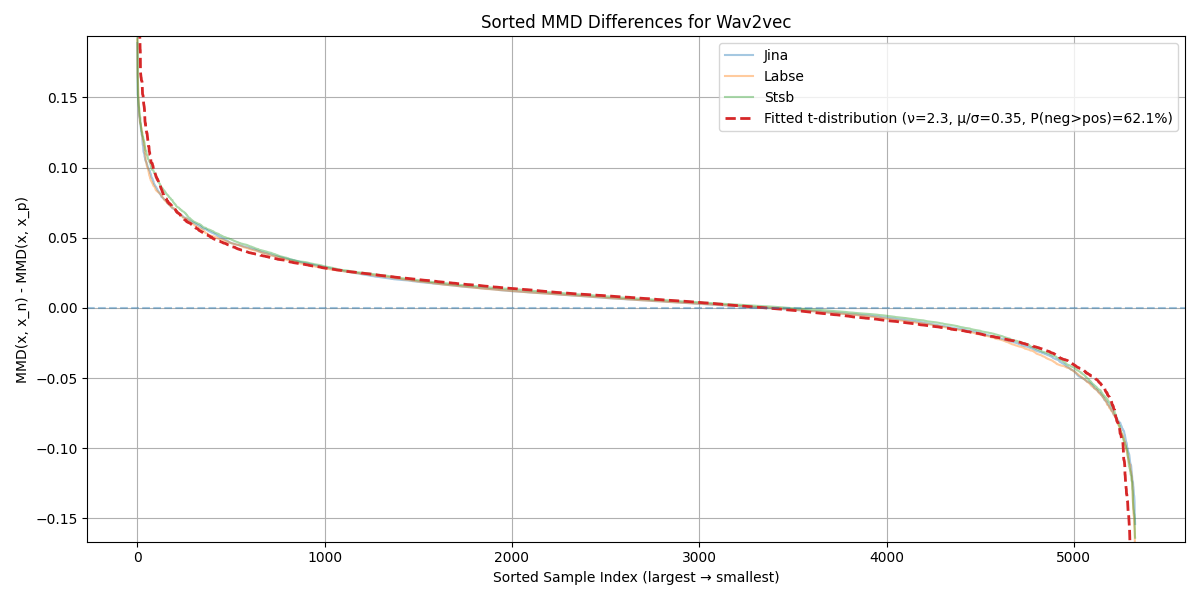
\includegraphics[width=0.8\linewidth]{figures/semantics/wav2vec.png}
    \caption{Rozkład wartości różnicy podobieństw dla Wav2Vec w ramach zbioru \textit{Medical Speech, Transcription, and Intent}}
    \label{fig:latent:medicalWav2Vec}
\end{figure}

\begin{figure}
    \centering
    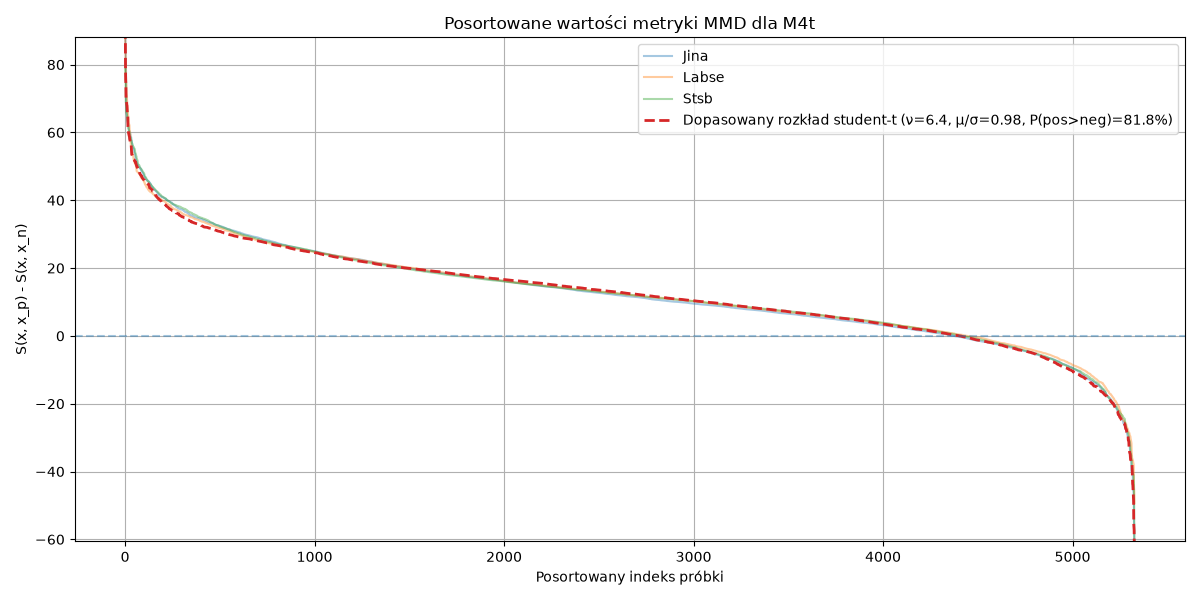
\includegraphics[width=0.8\linewidth]{figures/semantics/m4t_hani.png}
    \caption{Rozkład wartości różnicy podobieństw dla M4T w ramach zbioru \textit{Medical Speech, Transcription, and Intent}}
    \label{fig:latent:medicalM4T}
\end{figure}

\begin{figure}
    \centering
    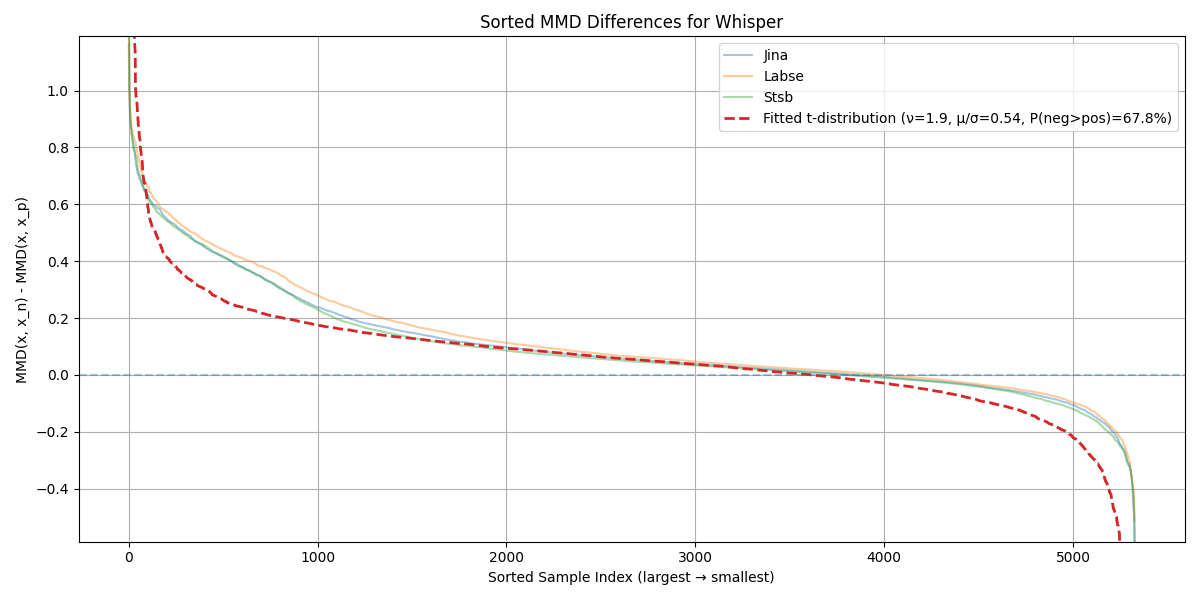
\includegraphics[width=0.8\linewidth]{figures/semantics/whisper.png}
    \caption{Rozkład wartości różnicy podobieństw dla Whisper w ramach zbioru \textit{Medical Speech, Transcription, and Intent}}
    \label{fig:latent:medicalWhisper}
\end{figure}

\begin{figure}
    \centering
    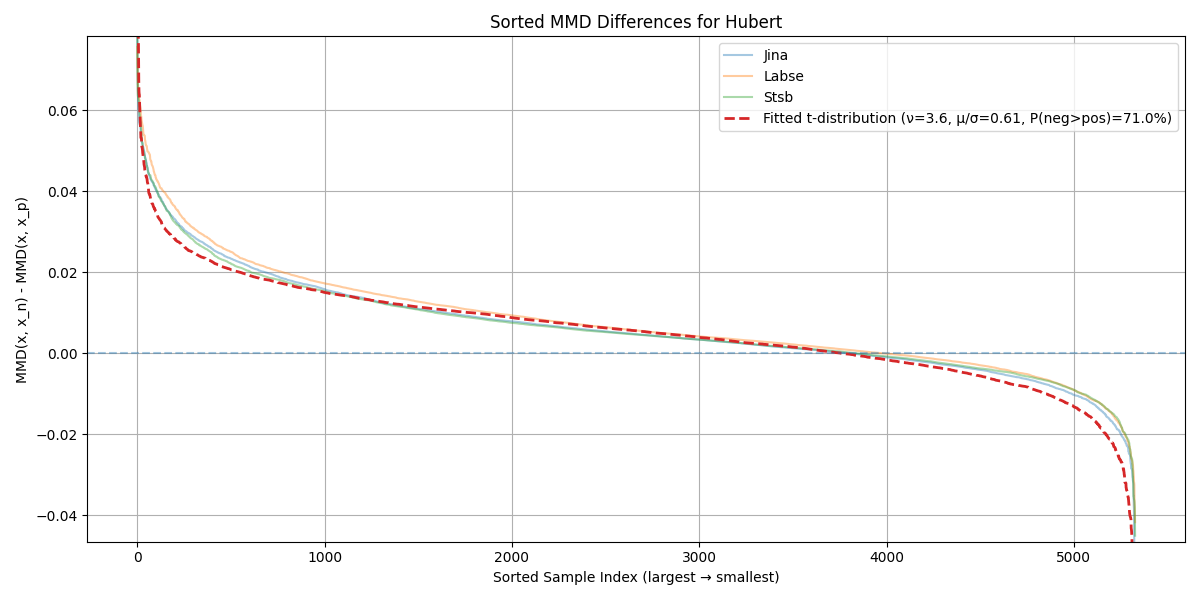
\includegraphics[width=0.8\linewidth]{figures/semantics/hubert.png}
    \caption{Rozkład wartości różnicy podobieństw dla Hubert w ramach zbioru \textit{Medical Speech, Transcription, and Intent}}
    \label{fig:latent:medicalHubert}
\end{figure}

\begin{figure}
    \centering
    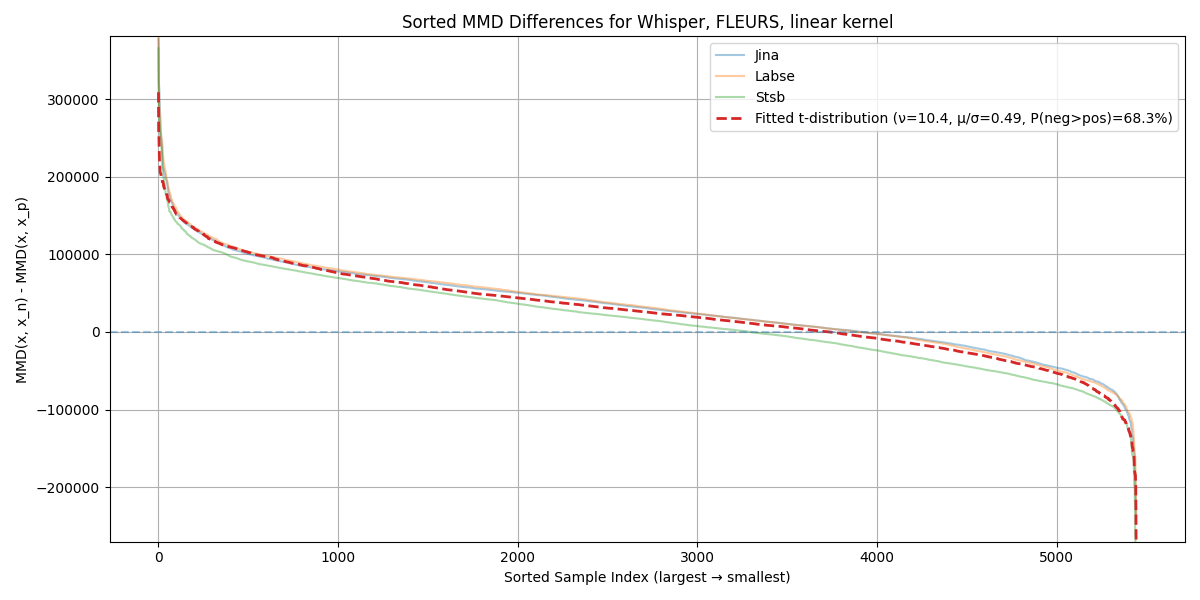
\includegraphics[width=0.8\linewidth]{figures/semantics/whisper_fleurs_linear.png}
    \caption{Rozkład wartości różnicy podobieństw dla Whisper w ramach zbioru \textit{Fleurs}}
    \label{fig:latent:fleursWhisper}
\end{figure}

\begin{figure}
    \centering
    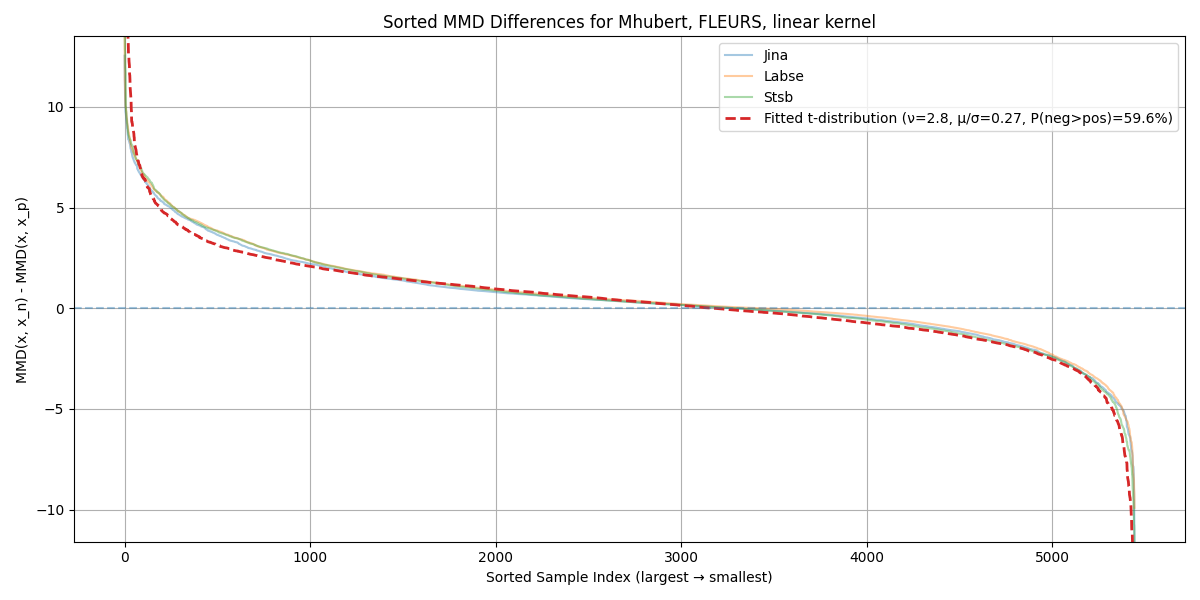
\includegraphics[width=0.8\linewidth]{figures/semantics/mhubert_fleurs_linear.png}
    \caption{Rozkład wartości różnicy podobieństw dla mHuBERT w ramach zbioru \textit{Fleurs}}
    \label{fig:latent:fleursMHubert}
\end{figure}

\begin{figure}
    \centering
    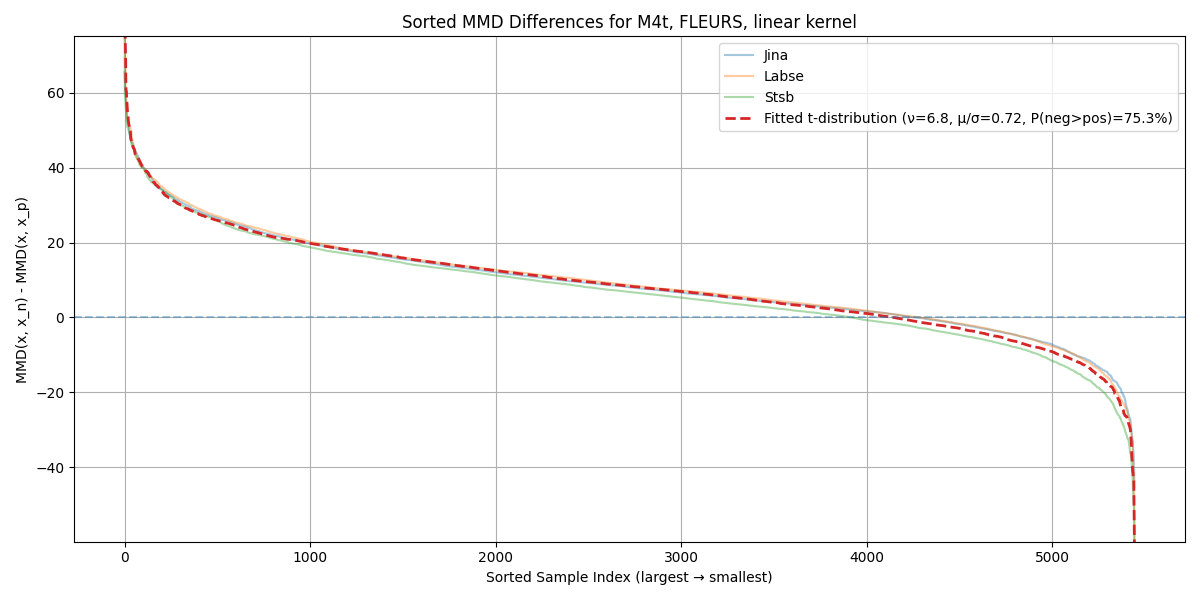
\includegraphics[width=0.8\linewidth]{figures/semantics/m4t_fleurs_linear.png}
    \caption{Rozkład wartości różnicy podobieństw dla M4T w ramach zbioru \textit{Fleurs}}
    \label{fig:latent:fleursM4T}
\end{figure}

\begin{figure}
    \centering
    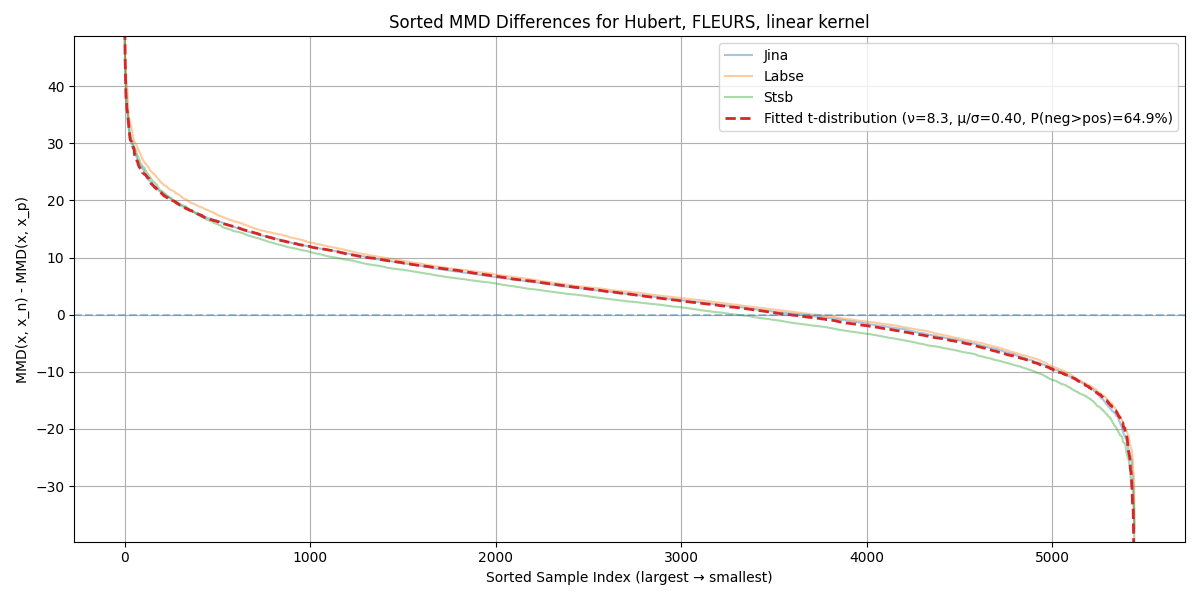
\includegraphics[width=0.8\linewidth]{figures/semantics/hubert_fleurs_linear.png}
    \caption{Rozkład wartości różnicy podobieństw dla HuBERT w ramach zbioru \textit{Fleurs}}
    \label{fig:latent:fleursHubert}
\end{figure}

\FloatBarrier


\subsection*{Analiza wpływu przetwarzania embeddingów na zachowanie semantyki}

\begin{figure}[!htbp]
    \centering
    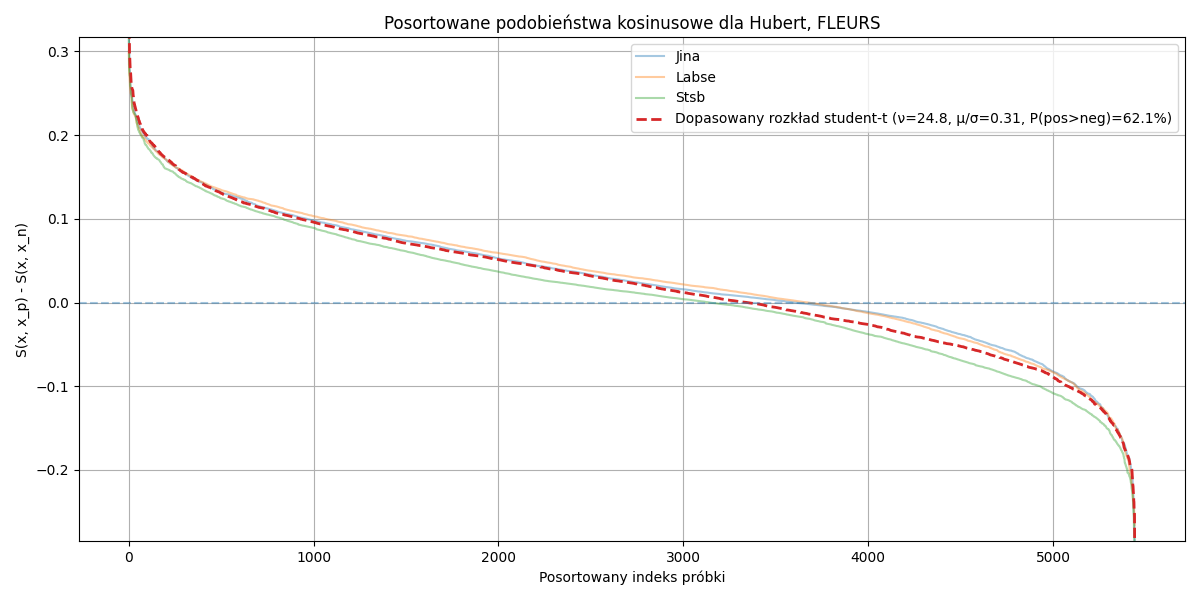
\includegraphics[width=0.8\linewidth]{figures/semantics/hubert_fleurs_linear_cosine.png}
    \caption{Rozkład wartości różnicy podobieństw dla HuBERT w ramach zbioru \textit{Fleurs}, \textit{mean pooling}}
    \label{fig:latent:simHubert}
\end{figure}

\begin{figure}[!htbp]
    \centering
    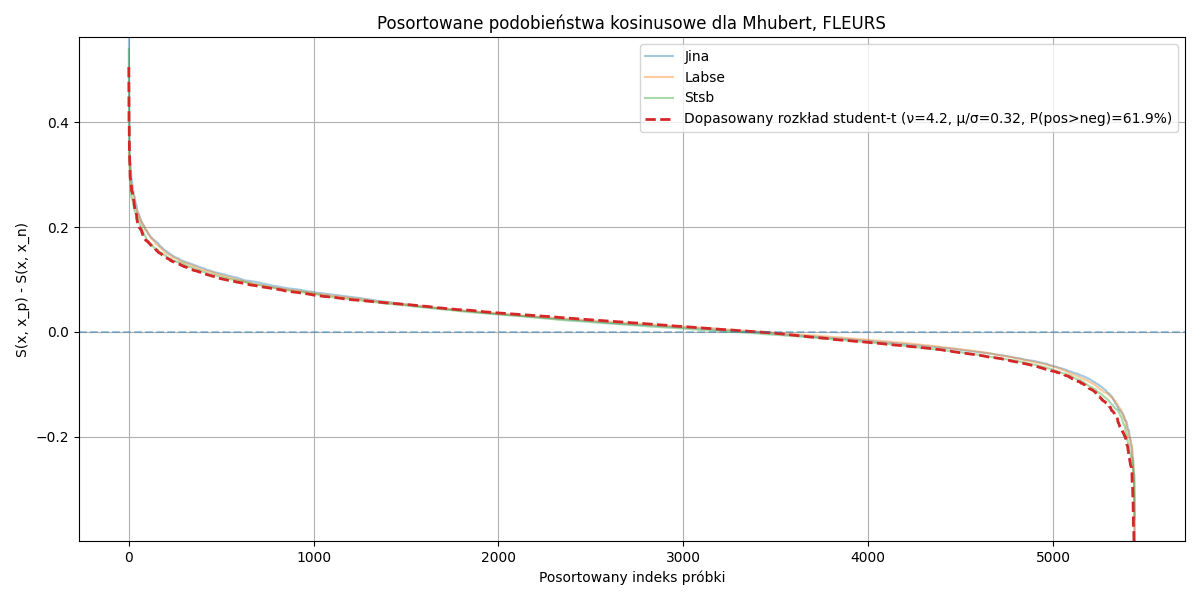
\includegraphics[width=0.8\linewidth]{figures/semantics/mhubert_fleurs_linear_cosine.png}
    \caption{Rozkład wartości różnicy podobieństw dla mHuBERT w ramach zbioru \textit{Fleurs}, \textit{mean pooling}}
    \label{fig:latent:simMhubert}
\end{figure}

\begin{figure}[!htbp]
    \centering
    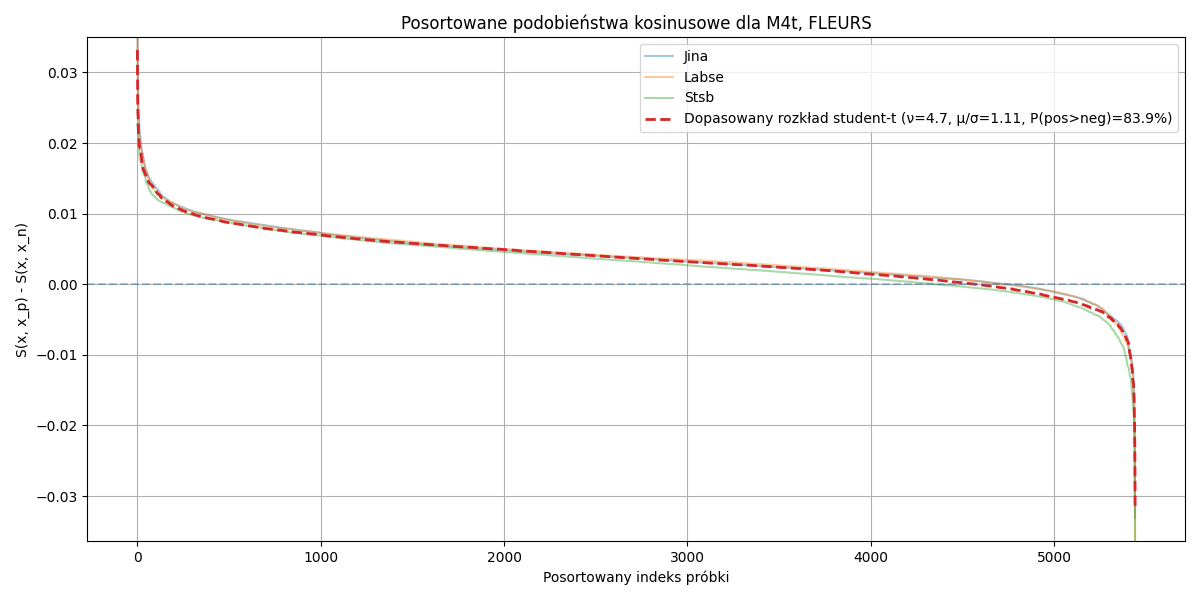
\includegraphics[width=0.8\linewidth]{figures/semantics/m4t_fleurs_linear_cosine.png}
    \caption{Rozkład wartości różnicy podobieństw dla SeamlessM4T w ramach zbioru \textit{Fleurs}, \textit{mean pooling}}
    \label{fig:latent:simM4T}
\end{figure}

\begin{figure}
    \centering
    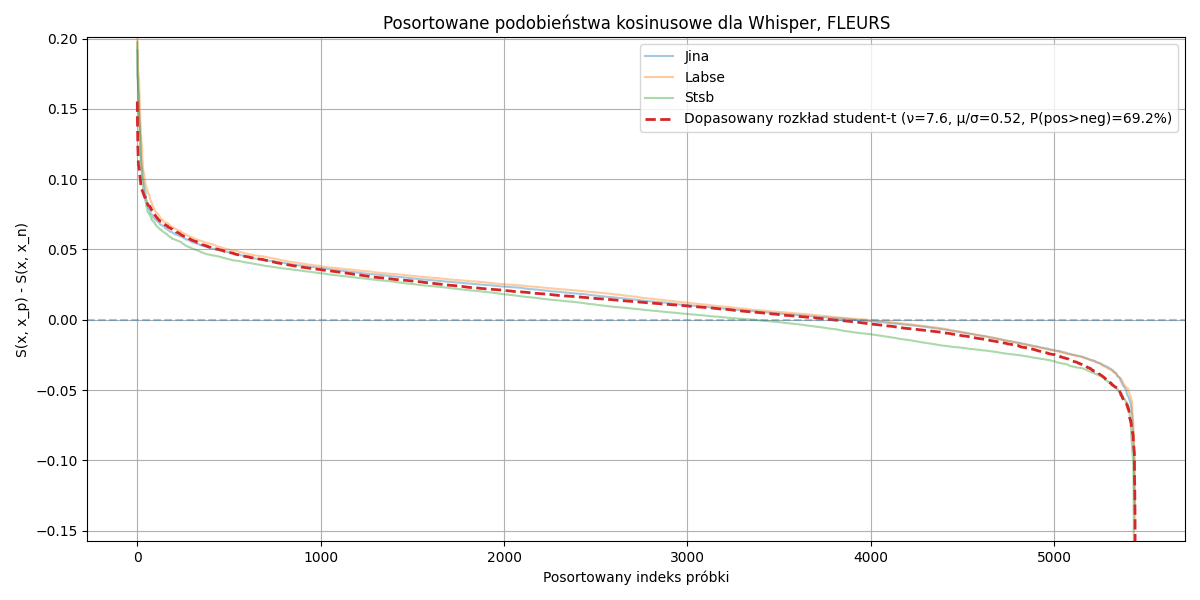
\includegraphics[width=0.8\linewidth]{figures/semantics/whisper_fleurs_linear_cosine.png}
    \caption{Rozkład wartości różnicy podobieństw dla Whisper w ramach zbioru \textit{Fleurs}, \textit{mean pooling}}
    \label{fig:latent:simWhisper}
\end{figure}


\begin{figure}
    \centering
    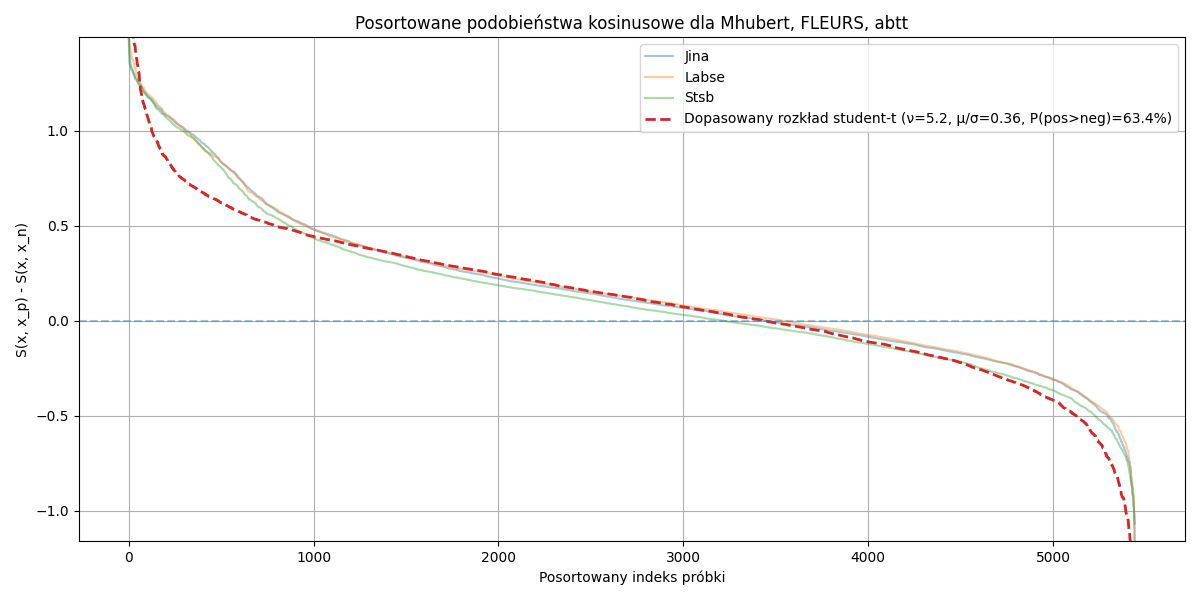
\includegraphics[width=0.8\linewidth]{figures/semantics/mhubert_fleurs_linear_abtt.png}
    \caption{Rozkład wartości różnicy podobieństw dla mHuBERT w ramach zbioru \textit{Fleurs}, \textit{mean pooling}, ABTT}
    \label{fig:latent:simMHubertAbtt}
\end{figure}

\begin{figure}
    \centering
    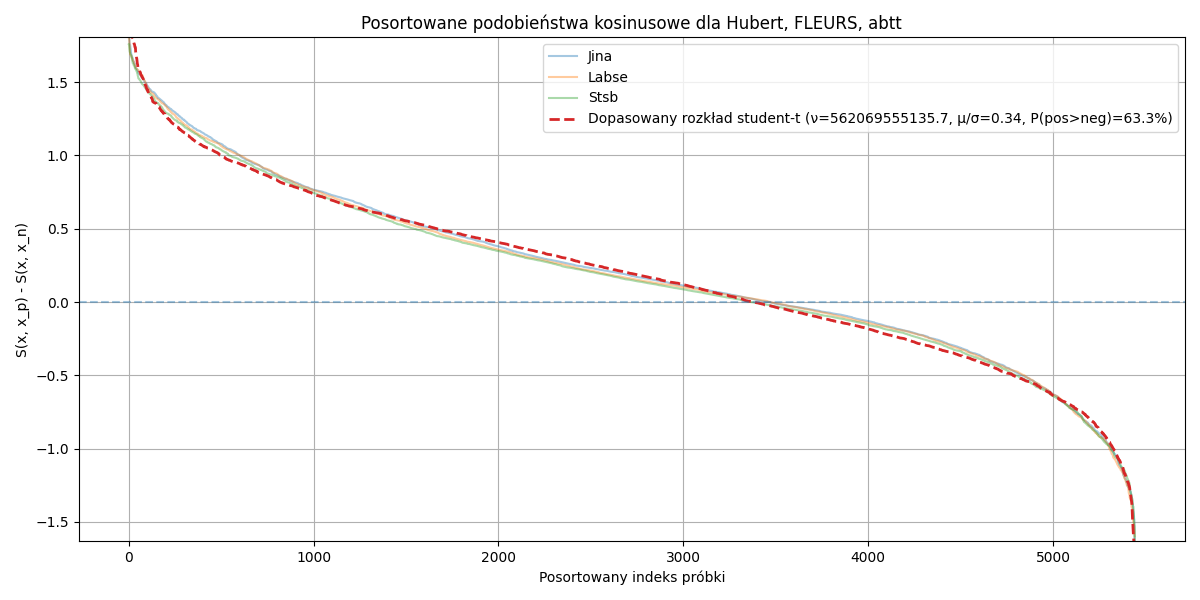
\includegraphics[width=0.8\linewidth]{figures/semantics/hubert_fleurs_linear_abtt.png}
    \caption{Rozkład wartości różnicy podobieństw dla HuBERT w ramach zbioru \textit{Fleurs}, \textit{mean pooling}, ABTT}
    \label{fig:latent:simHubertAbtt}
\end{figure}

\begin{figure}
    \centering
    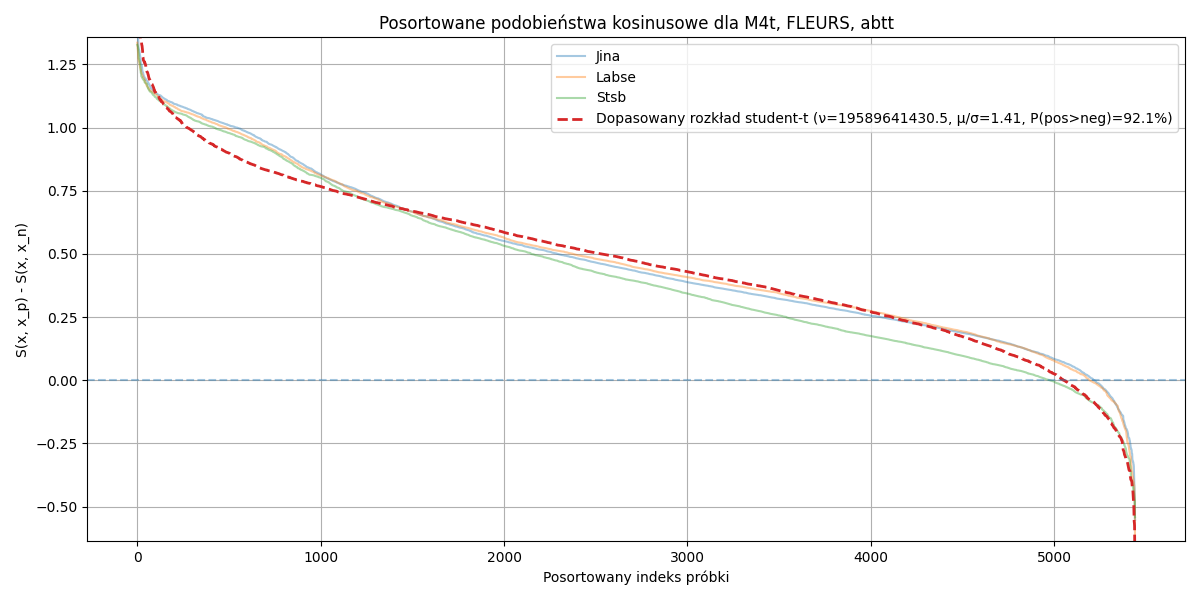
\includegraphics[width=0.8\linewidth]{figures/semantics/m4t_fleurs_linear_abtt.png}
    \caption{Rozkład wartości różnicy podobieństw dla SeamlessM4T w ramach zbioru \textit{Fleurs}, \textit{mean pooling}, ABTT}
    \label{fig:latent:simM4TAbtt}
\end{figure}

\begin{figure}
    \centering
    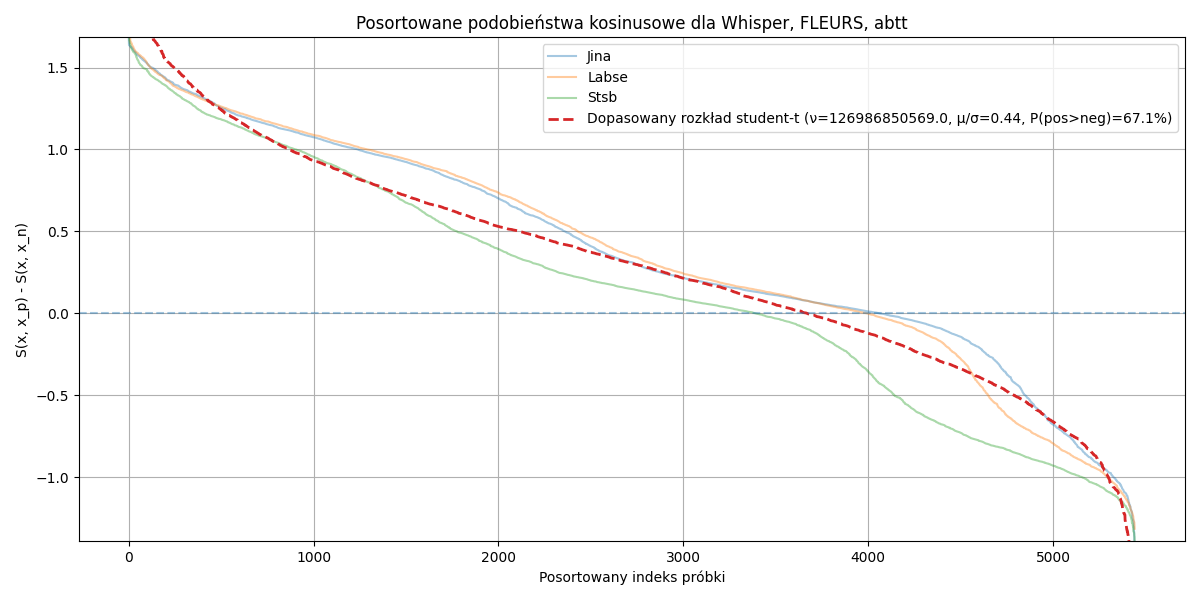
\includegraphics[width=0.8\linewidth]{figures/semantics/whisper_fleurs_linear_abtt.png}
    \caption{Rozkład wartości różnicy podobieństw dla Whisper w ramach zbioru \textit{Fleurs}, \textit{mean pooling}, ABTT}
    \label{fig:latent:simWhisperAbtt}
\end{figure}
